\subsection{IEEE 1451}
O IEEE 1451 se divide em uma família de padrões que foram criados com os objetivos de permitir a capacidade de comunicação entre transdutores(sensores e atuadores) de forma \emph{plug-and-play} por meio de redes com ou sem fio, facilitar a criação de transdutores com inteligência embarcada, simplificar a configuração e manutenção de sistemas, prover comunicação entre transdutores legados, e por fim, habilitar a implementação de transdutores inteligentes e com uso mínimo de memória~\cite{ieee1451journal}.

Um dos padrões da família, o IEEE 1451.1, define um modelo de informação para \emph{Network Capable Application Processors} (NCAP) que foi estabelecido para especificar um modelo de objetos comum e interfaces de componentes da rede de transdutores. Dessa forma, foi desenvolvido um \emph{framework} orientado a objetos que pode ser estendido para facilitar o desenvolvimento de aplicações que foi definido da seguinte forma: Um modelo de dados que especifica a forma e o tipo de comunicação, tanto local quanto remota, por meio das interfaces de objetos 1451.1, um modelo de objetos que especifica tipos de componentes de software usados para definir e implementar sistemas e, por fim, modelos de comunicação que definem a sintaxe e semântica das interfaces de software entre redes de comunicação e objetos de aplicação~\cite{ieeeOO1451}~\cite{ieee1451monitoring}.

\begin{figure}[ht]
\center
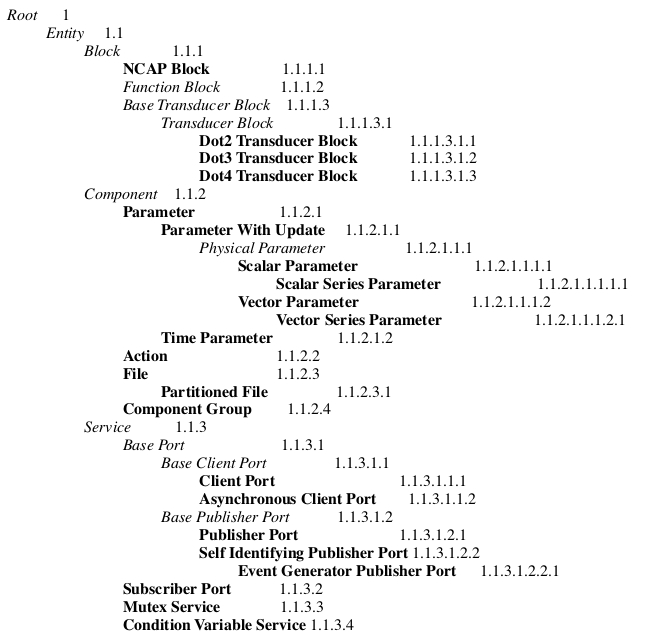
\includegraphics[scale=0.5]{imagens/ieee1451-classHierarchy}
\caption{Hierarquia de Classes do Padrão IEEE 1451.1}
\label{fig:classHierarchy}
\end{figure}

O padrão ~\cite{ieee1451standard} especifica cada classe no modelo definindo as interfaces da classe(por meio de assinaturas e operações) e o comportamento da classe (via texto ou máquinas de estado). A figura~\ref{fig:classHierarchy} mostra a hierarquia de classes definida pelo padrão em que as classes em itálico representam classes abstratas. Nesta figura é possível observar 3 tipos principais de objetos IEEE 1451.1:

\begin{itemize}
	\item\emph{Block}:

	Especializada em três classes:
		\begin{itemize}
			\item\emph{NCAPBlock}:
				Provê interfaces para comunicações de rede e configurações do sistema.
			\item\emph{BaseTransducerBlock}:
				Provê interfaces entre transdutores e funções.
			\item\emph{FunctionBlock}:
				Provê encapsulamento de funções específicas.
		\end{itemize}
	
	\item\emph{Component}:
	
		Fornecem:
		\begin{itemize}
			\item Informações estruturadas: medidas e arquivos.
			\item Coleções de objetos relacionados com a aplicação.
			\item Ações com estados onde a ação é executada após um período de tempo.
		\end{itemize}
	\item\emph{Service}:
	
		Suportam:
		\begin{itemize}
			\item Comunicação entre objetos de diferentes NCAPs.
			\item Sincronização do sistema.
		\end{itemize}
\end{itemize}

Há ainda as classes não-IEEE 1451.1, que não estão representadas na Figura ~\ref{fig:classHierarchy} e possuem restrições de aplicabilidade na arquitetura IEEE 1451.


